\begin{block}{house elevation}
    Households elevate their homes to manage flood risks, but regulations and guidance are silent on key questions \cite{zarekarizi_suboptimal:2020,xian_elevation:2017}.
    \begin{framed}
        \begin{description}
            \item[Q1] How to adapt guidance to building characteristics or household preferences?
            \item[Q2] How does nonstationary hazard change guidance?
            \item[Q3] Which model of nonstationary hazard should be used?
        \end{description}
    \end{framed}
    \begin{figure}
        \centering
        \subcaptionbox{Selinsgrove, PA}{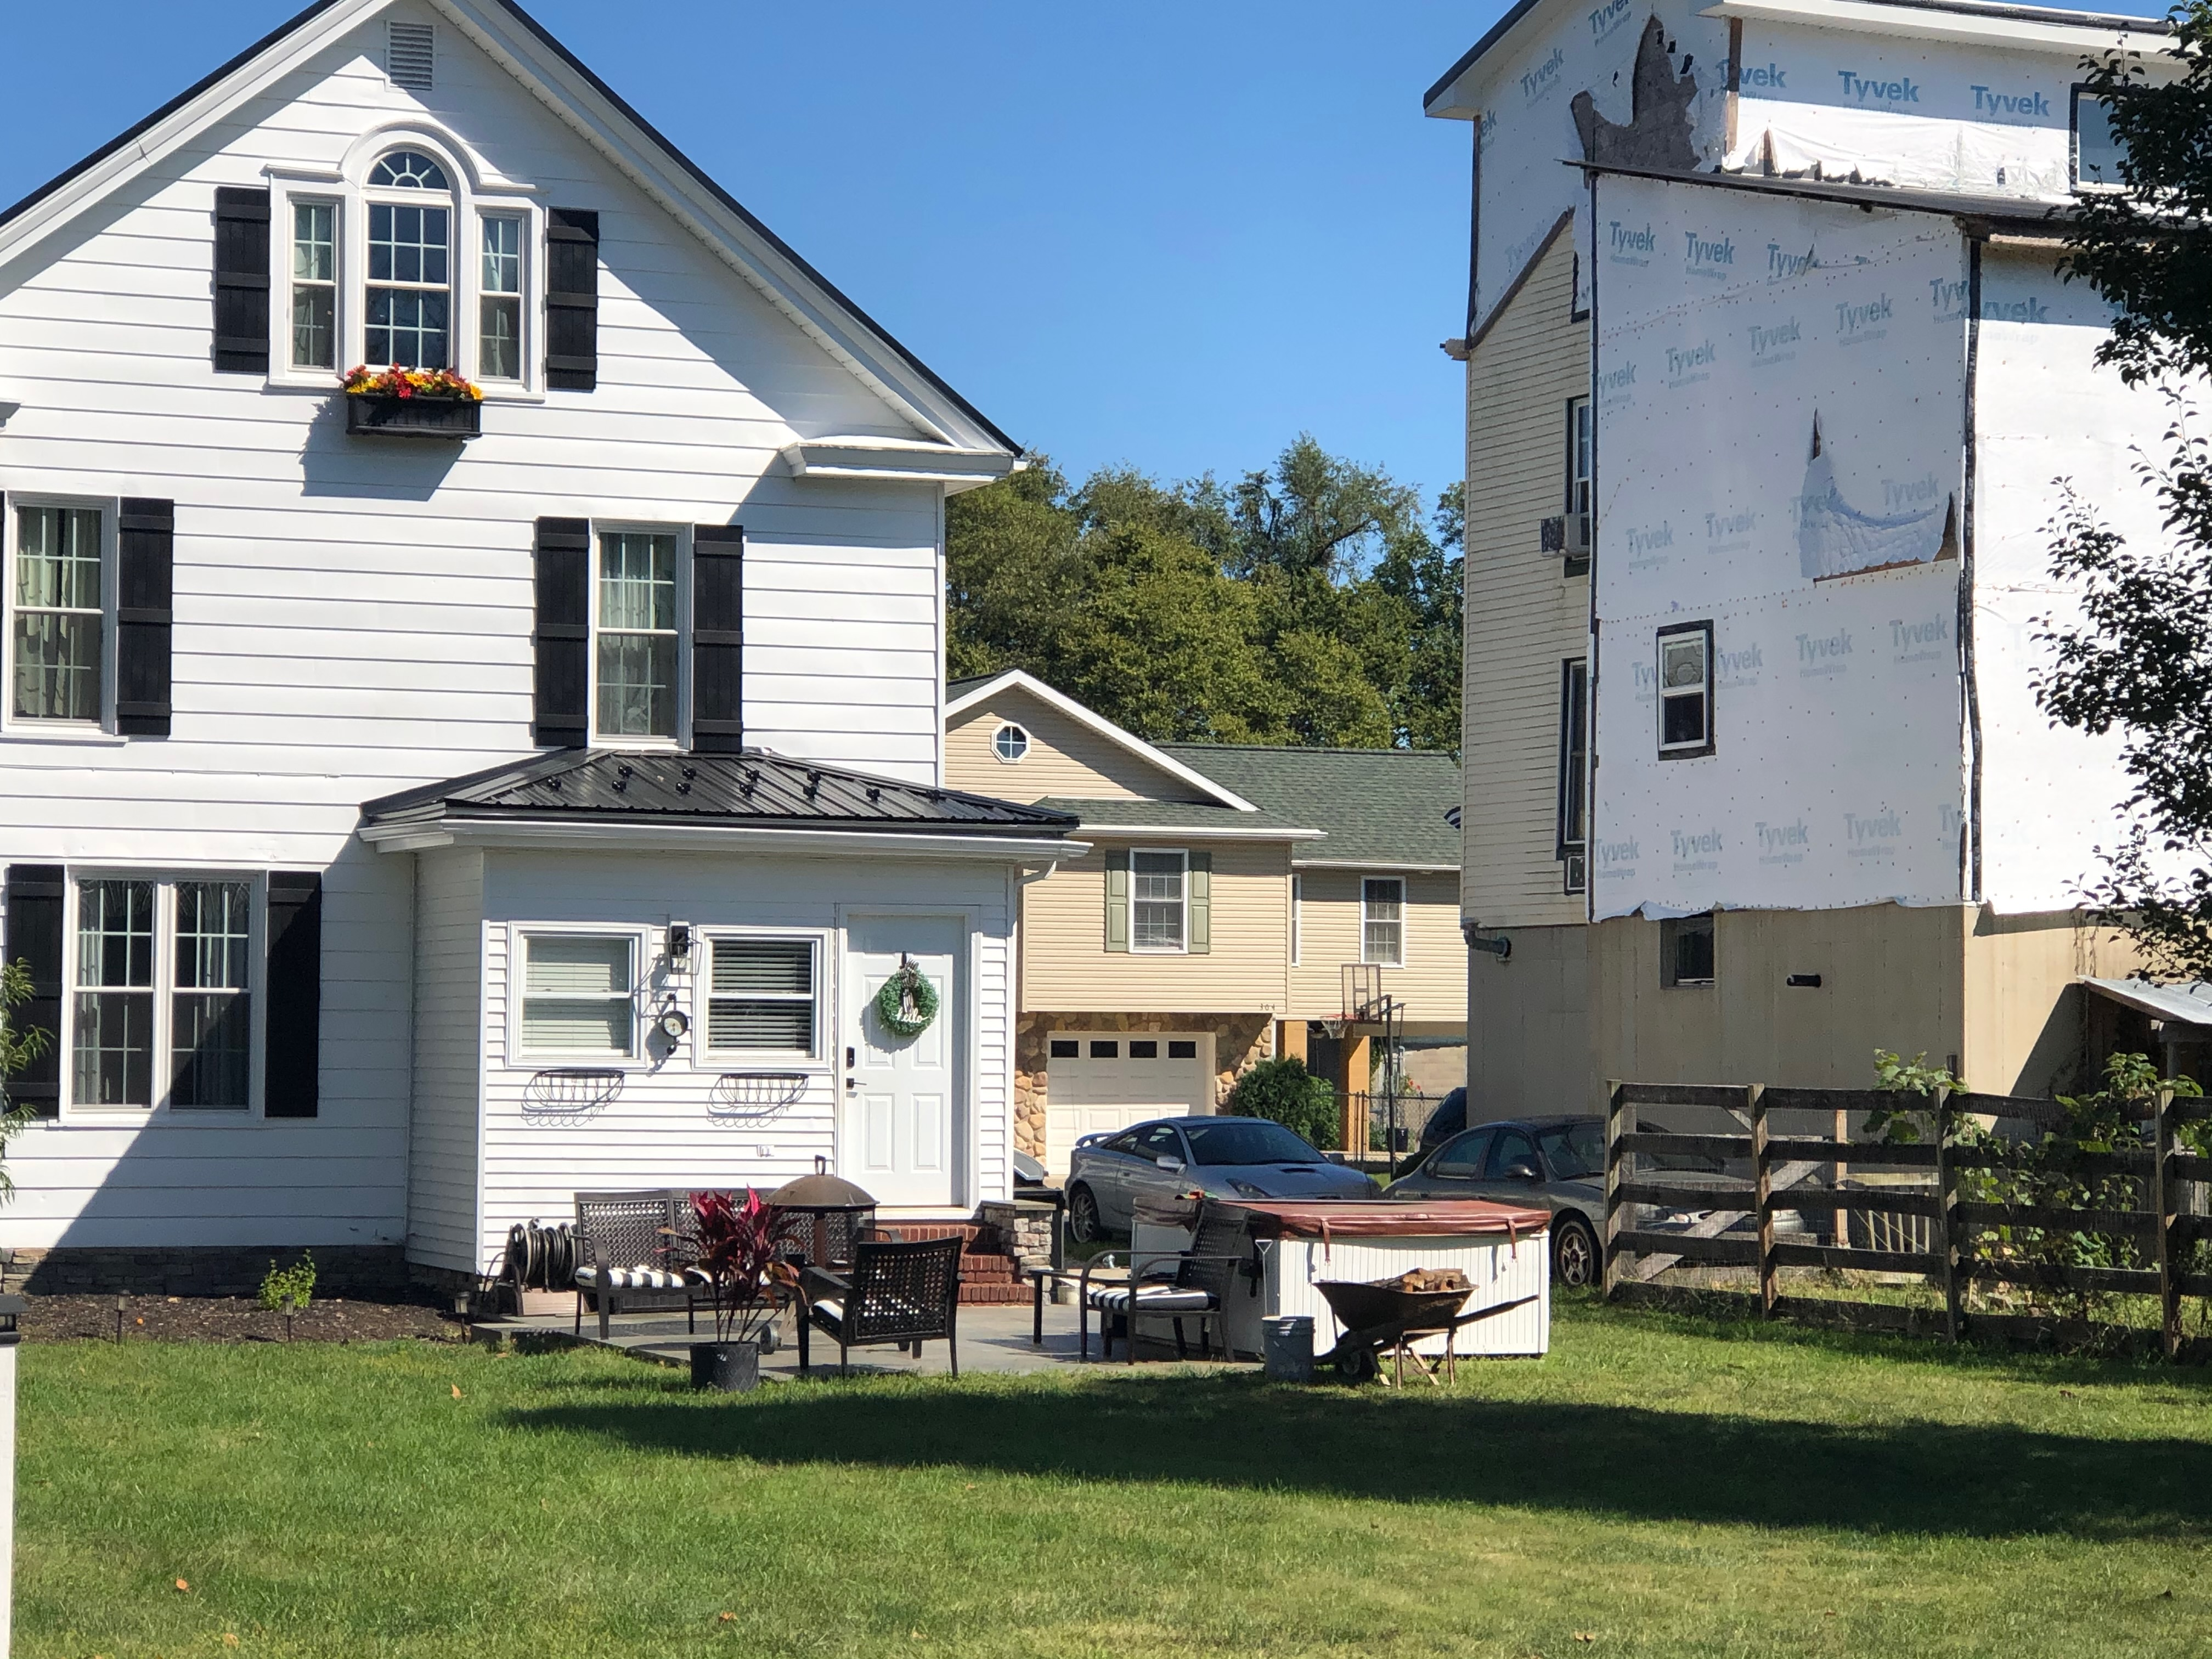
\includegraphics[height=3.35in]{img_selinsgrove.jpeg}}%
        \hfill
        \subcaptionbox{Houston, TX}{\includegraphics[height=3.35in]{img_braeswood.png}}\\
        \subcaptionbox{Plaquemines Parish, LA}{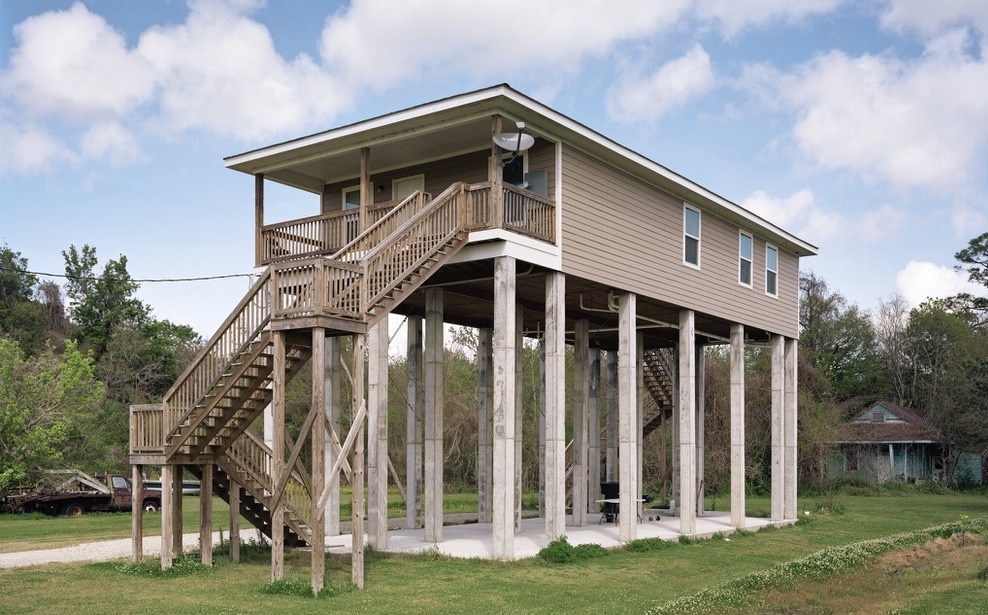
\includegraphics[height=3.3in]{epstein-2020-la.jpeg}}%
        \hfill
        \subcaptionbox{Dare County, NC}{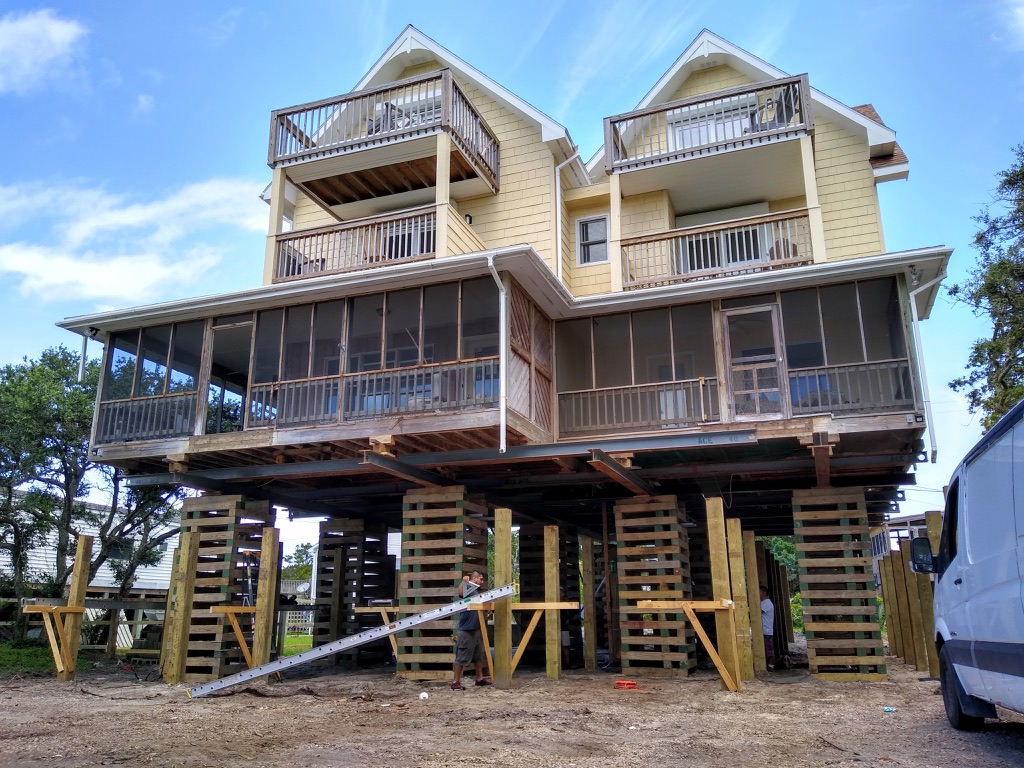
\includegraphics[height=3.3in]{nichols-ocracoke.jpeg}}%
        \caption{
            \faIcon{camera}: (a) JDG, (b) Google Maps, (c) Mitch Epstein /  New York Times (d) Rob Nichols.
        }
        \label{fig:images}
    \end{figure}
\end{block}